\documentclass{beamer}
\usetheme{CambridgeUS}
\title[Process]{A numerical evaluation of the Koopman operator}
\subtitle{Prediction error over the forced Van Der Pol oscillator}
\institute[Polimi]{Politecnico di Milano}
\author{Sergio Vanegas}
\date{\today}

\usepackage{siunitx}
\usepackage{csvsimple}

\usepackage{caption}
\usepackage{subcaption}

\begin{document}

\begin{frame}[plain,noframenumbering]
    \maketitle
\end{frame}

\begin{frame}{Table of Contents}
    \tableofcontents
\end{frame}


\section{Introduction}

\begin{frame}{Introduction}
    \footnotesize
    In this document, a numerical evaluation of the accuracy of the Koopman operator in its current implementation is presented. The centers are now taken from random snapshots in the dataset\footnote{Some centers had to be restored to fully random because of noticeably higher error results}, but the Koopman matrix projection algorithm was modified so that the optimization problems would minimize over the average instead of the total squared error, avoiding numerical overflow for larger datasets.

    The signals used for the input were the following:

    \begin{itemize}
        \item Steady 0-input.
        \item Sine input of $2$ Hz.
        \item Square input generated by  applying the sign function to the sine wave.
    \end{itemize}
    
    The result tables are classified by input signal, prediction horizon, and presence of noise in the training data. Each table is organized in columns by regularization coefficient and in rows by observable order. 
    
    All error values are presented as a percentage, and correspond to the normalized trajectory prediction error averaged over a thousand different trajectories for each parameter combination.

    Following the result tables, a set of conclusions is included.
\end{frame}


\section{Prediction error - Steady input}

\begin{frame}{Steady input - $0.25$ seconds}
    \scriptsize
    \begin{table}[!ht]
        \centering
        \csvautotabular{Tables_Clean/table_steady_T_0.25.csv}
        \caption{Clean Training Data}
    \end{table}

    \begin{table}[!ht]
        \centering
        \csvautotabular{Tables_Noisy/table_steady_T_0.25.csv}
        \caption{Noisy Training Data}
    \end{table}
\end{frame}

\begin{frame}{Steady input - $0.50$ seconds}
    \scriptsize
    \begin{table}[!ht]
        \centering
        \csvautotabular{Tables_Clean/table_steady_T_0.50.csv}
        \caption{Clean Training Data}
    \end{table}

    \begin{table}[!ht]
        \centering
        \csvautotabular{Tables_Noisy/table_steady_T_0.50.csv}
        \caption{Noisy Training Data}
    \end{table}
\end{frame}

\begin{frame}{Steady input - $1.00$ seconds}
    \scriptsize
    \begin{table}[!ht]
        \centering
        \csvautotabular{Tables_Clean/table_steady_T_1.00.csv}
        \caption{Clean Training Data}
    \end{table}

    \begin{table}[!ht]
        \centering
        \csvautotabular{Tables_Noisy/table_steady_T_1.00.csv}
        \caption{Noisy Training Data}
    \end{table}
\end{frame}

\begin{frame}{Steady input - Figures}
    \begin{figure}
        \centering
        \begin{subfigure}[b]{0.3\textwidth}
            \centering
            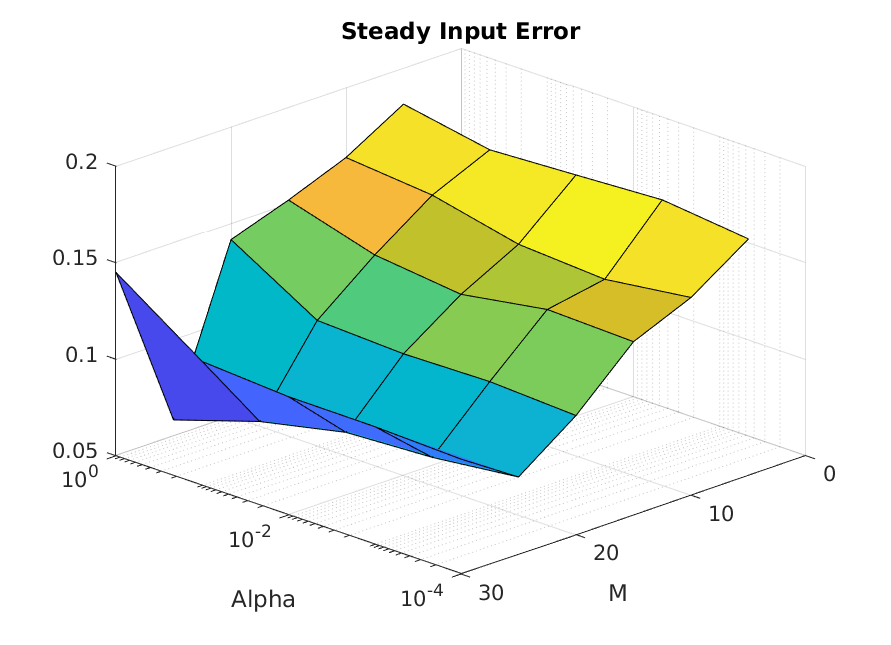
\includegraphics[width=\textwidth]{Figures_Clean/figure_steady_T_0.25.png}
            \caption{Clean - 0.25 s}
            \label{fig:clean_steady_025}
        \end{subfigure}
        \hfill
        \begin{subfigure}[b]{0.3\textwidth}
            \centering
            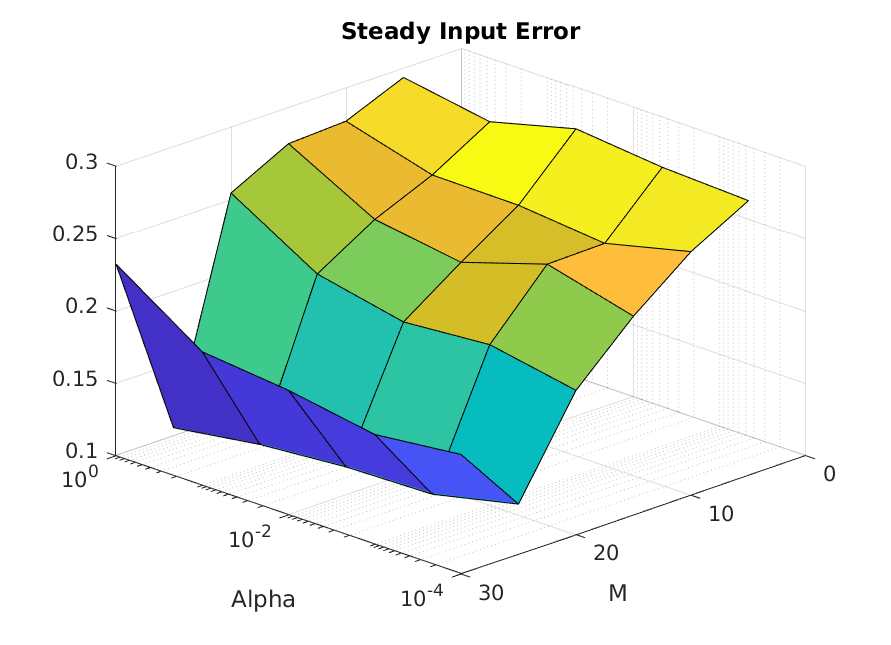
\includegraphics[width=\textwidth]{Figures_Clean/figure_steady_T_0.50.png}
            \caption{Clean - 0.50 s}
            \label{fig:clean_steady_050}
        \end{subfigure}
        \hfill
        \begin{subfigure}[b]{0.3\textwidth}
            \centering
            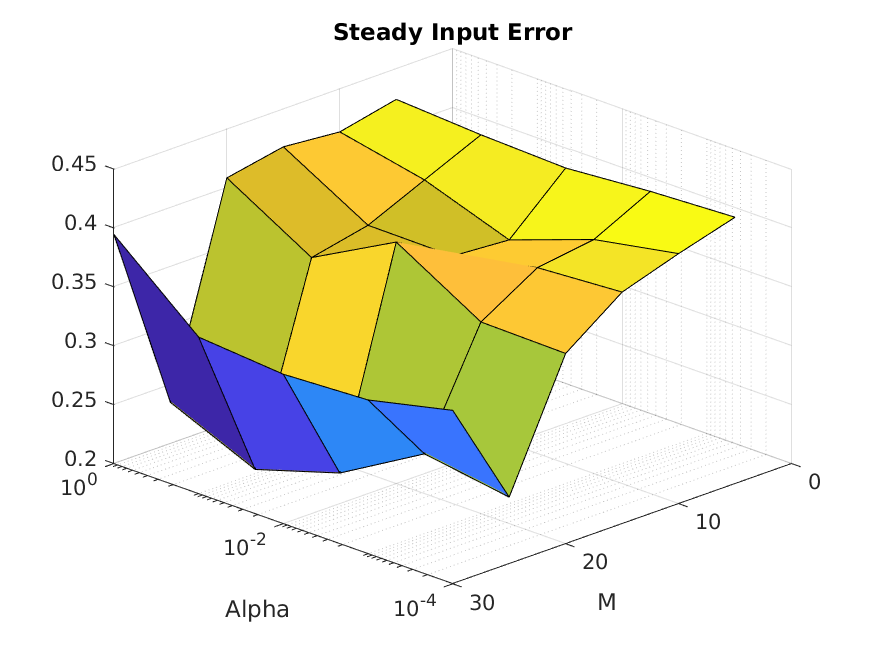
\includegraphics[width=\textwidth]{Figures_Clean/figure_steady_T_1.00.png}
            \caption{Clean - 1.00 s}
            \label{fig:clean_steady_100}
        \end{subfigure}
        \\
        \begin{subfigure}[b]{0.3\textwidth}
            \centering
            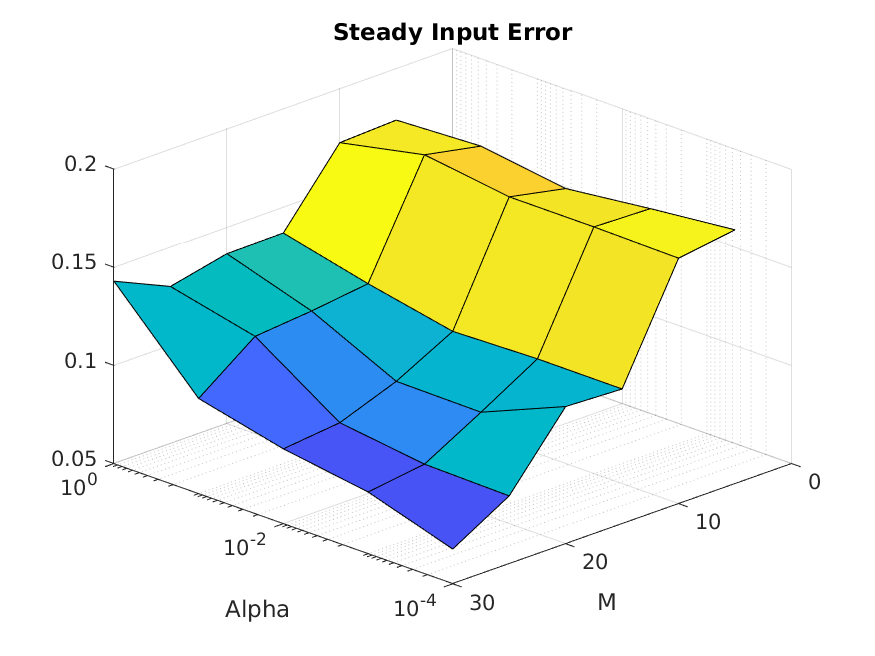
\includegraphics[width=\textwidth]{Figures_Noisy/figure_steady_T_0.25.png}
            \caption{Noisy - 0.25 s}
            \label{fig:noisy_steady_025}
        \end{subfigure}
        \hfill
        \begin{subfigure}[b]{0.3\textwidth}
            \centering
            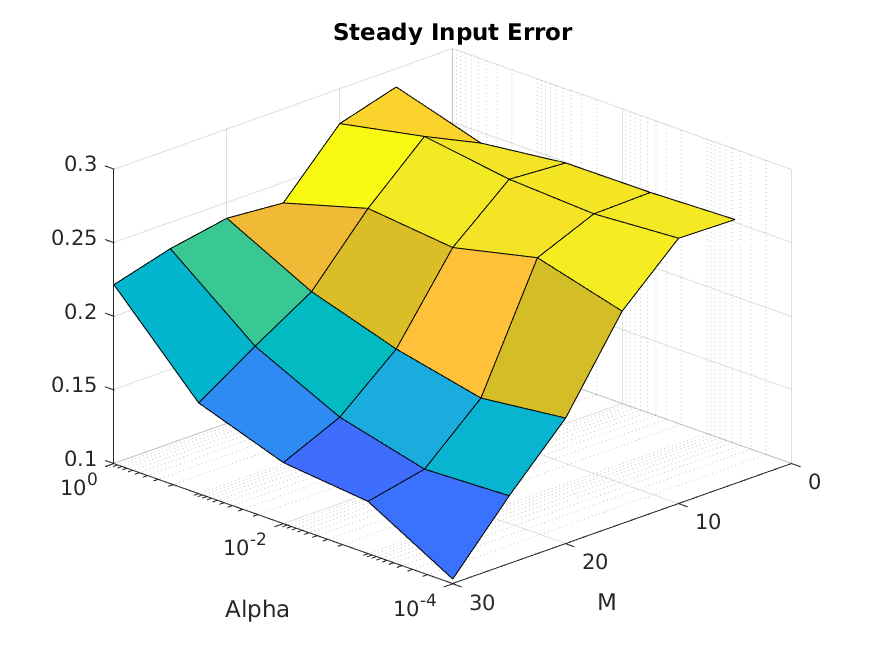
\includegraphics[width=\textwidth]{Figures_Noisy/figure_steady_T_0.50.png}
            \caption{Noisy - 0.50 s}
            \label{fig:noisy_steady_050}
        \end{subfigure}
        \hfill
        \begin{subfigure}[b]{0.3\textwidth}
            \centering
            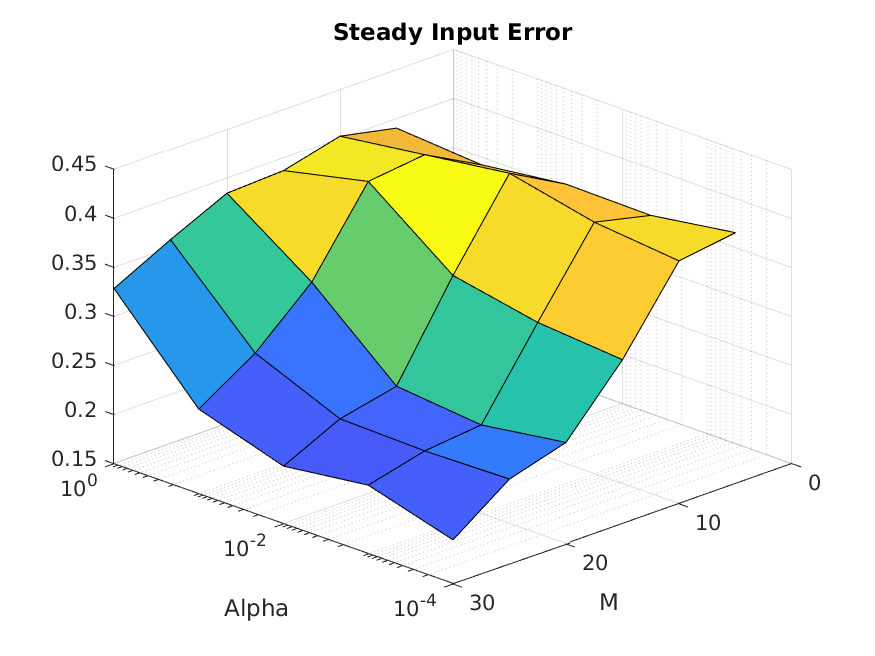
\includegraphics[width=\textwidth]{Figures_Noisy/figure_steady_T_1.00.png}
            \caption{Noisy - 1.00 s}
            \label{fig:noisy_steady_100}
        \end{subfigure}
        \label{fig:clean_steady}
    \end{figure}
\end{frame}


\section{Prediction error - Sine input}

\begin{frame}{Sine input - $0.25$ seconds}
    \scriptsize
    \begin{table}[!ht]
        \centering
        \csvautotabular{Tables_Clean/table_sine_T_0.25.csv}
        \caption{Clean Training Data}
    \end{table}

    \begin{table}[!ht]
        \centering
        \csvautotabular{Tables_Noisy/table_sine_T_0.25.csv}
        \caption{Noisy Training Data}
    \end{table}
\end{frame}

\begin{frame}{Sine input - $0.50$ seconds}
    \scriptsize
    \begin{table}[!ht]
        \centering
        \csvautotabular{Tables_Clean/table_sine_T_0.50.csv}
        \caption{Clean Training Data}
    \end{table}

    \begin{table}[!ht]
        \centering
        \csvautotabular{Tables_Noisy/table_sine_T_0.50.csv}
        \caption{Noisy Training Data}
    \end{table}
\end{frame}

\begin{frame}{Sine input - $1.00$ seconds}
    \scriptsize
    \begin{table}[!ht]
        \centering
        \csvautotabular{Tables_Clean/table_sine_T_1.00.csv}
        \caption{Clean Training Data}
    \end{table}

    \begin{table}[!ht]
        \centering
        \csvautotabular{Tables_Noisy/table_sine_T_1.00.csv}
        \caption{Noisy Training Data}
    \end{table}
\end{frame}

\begin{frame}{Sine input - Figures}
    \begin{figure}
        \centering
        \begin{subfigure}[b]{0.3\textwidth}
            \centering
            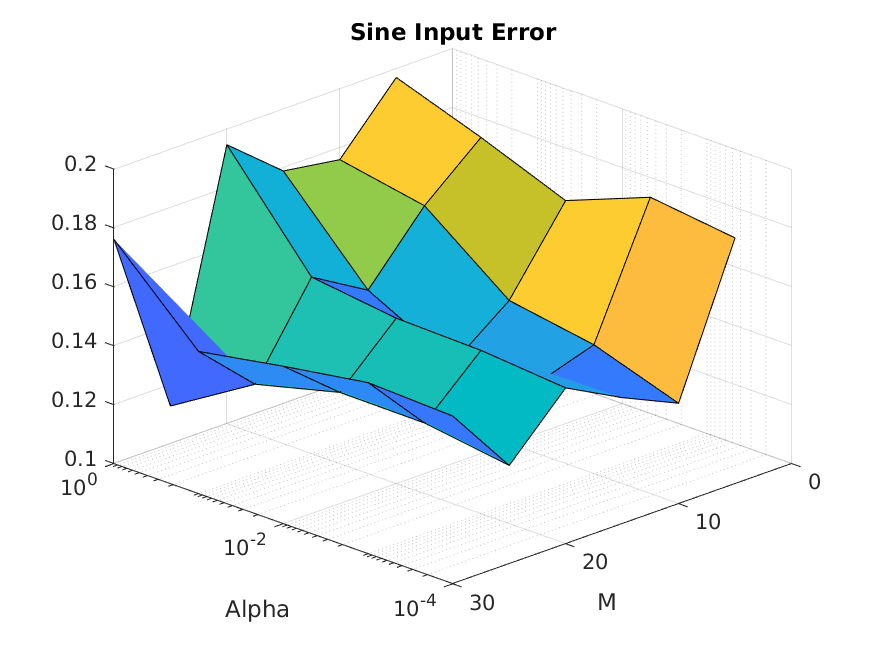
\includegraphics[width=\textwidth]{Figures_Clean/figure_sine_T_0.25.png}
            \caption{Clean - 0.25 s}
            \label{fig:clean_sine_025}
        \end{subfigure}
        \hfill
        \begin{subfigure}[b]{0.3\textwidth}
            \centering
            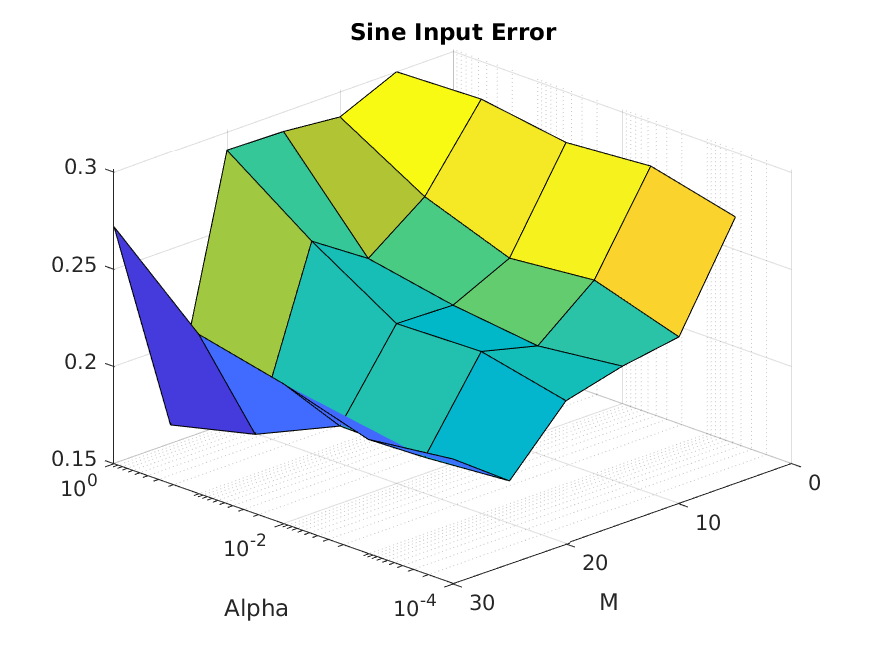
\includegraphics[width=\textwidth]{Figures_Clean/figure_sine_T_0.50.png}
            \caption{Clean - 0.50 s}
            \label{fig:clean_sine_050}
        \end{subfigure}
        \hfill
        \begin{subfigure}[b]{0.3\textwidth}
            \centering
            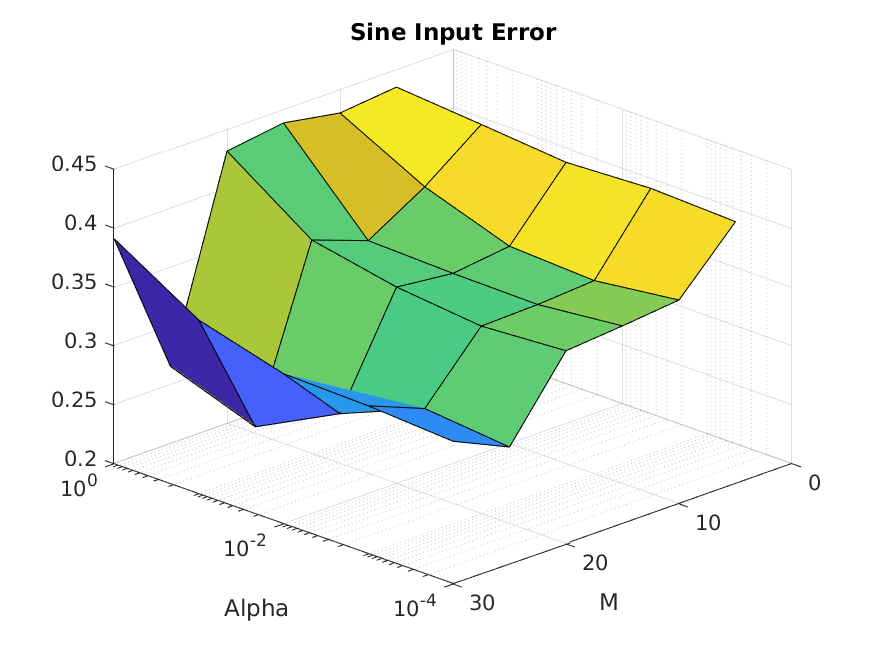
\includegraphics[width=\textwidth]{Figures_Clean/figure_sine_T_1.00.png}
            \caption{Clean - 1.00 s}
            \label{fig:clean_sine_100}
        \end{subfigure}
        \\
        \begin{subfigure}[b]{0.3\textwidth}
            \centering
            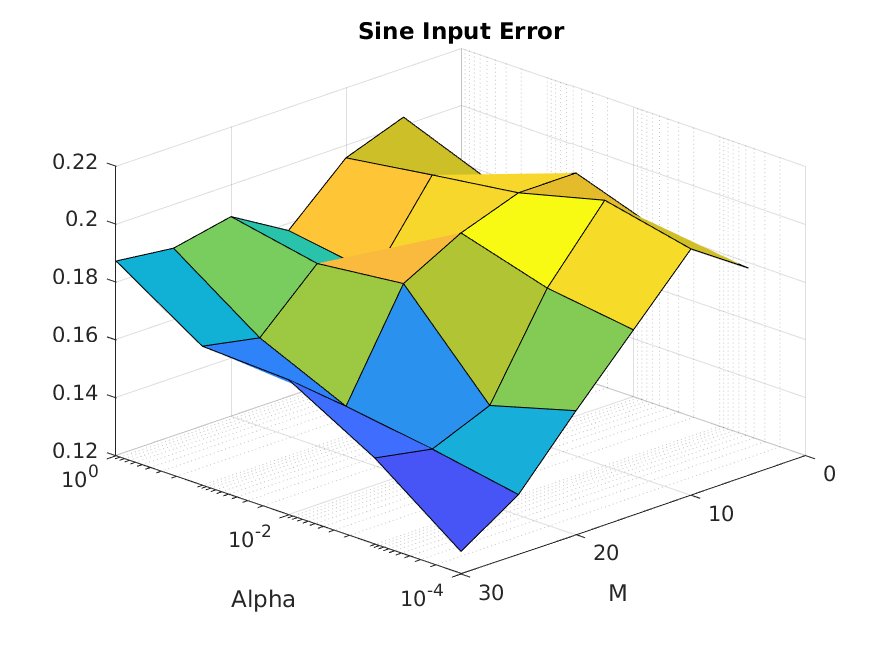
\includegraphics[width=\textwidth]{Figures_Noisy/figure_sine_T_0.25.png}
            \caption{Noisy - 0.25 s}
            \label{fig:noisy_sine_025}
        \end{subfigure}
        \hfill
        \begin{subfigure}[b]{0.3\textwidth}
            \centering
            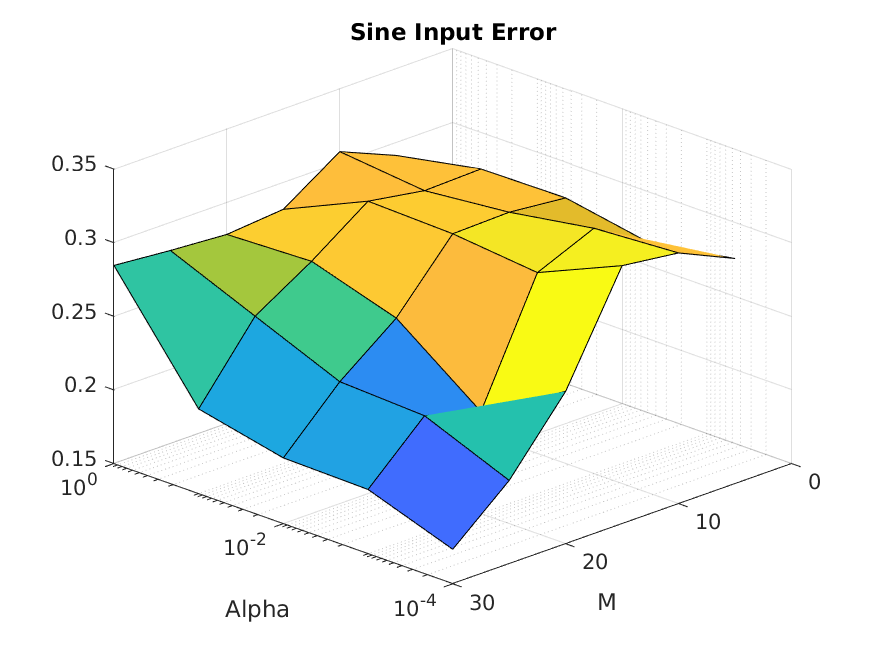
\includegraphics[width=\textwidth]{Figures_Noisy/figure_sine_T_0.50.png}
            \caption{Noisy - 0.50 s}
            \label{fig:noisy_sine_050}
        \end{subfigure}
        \hfill
        \begin{subfigure}[b]{0.3\textwidth}
            \centering
            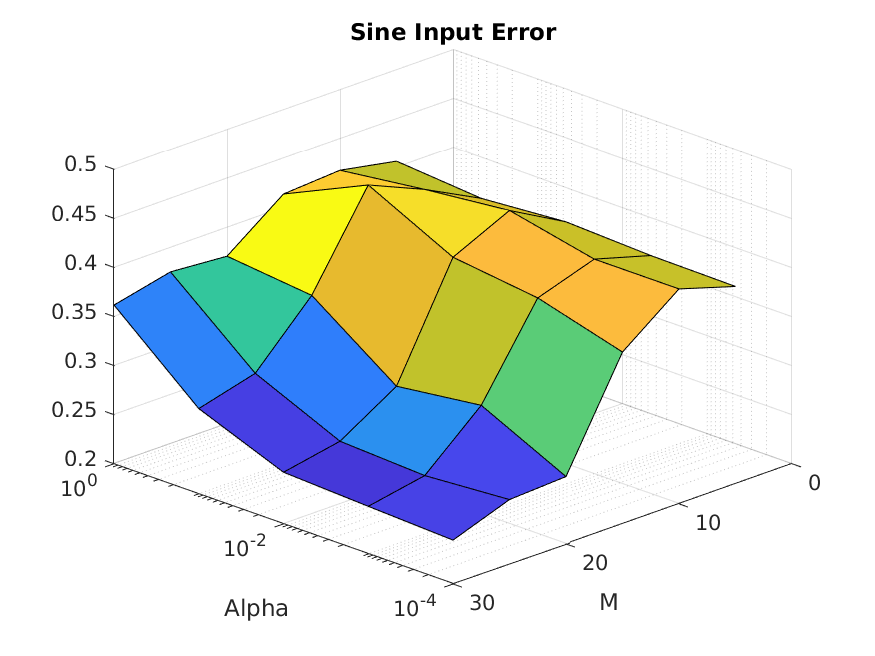
\includegraphics[width=\textwidth]{Figures_Noisy/figure_sine_T_1.00.png}
            \caption{Noisy - 1.00 s}
            \label{fig:noisy_sine_100}
        \end{subfigure}
        \label{fig:clean_sine}
    \end{figure}
\end{frame}


\section{Prediction error - Square input}

\begin{frame}{Square input - $0.25$ seconds}
    \scriptsize
    \begin{table}[!ht]
        \centering
        \csvautotabular{Tables_Clean/table_square_T_0.25.csv}
        \caption{Clean Training Data}
    \end{table}

    \begin{table}[!ht]
        \centering
        \csvautotabular{Tables_Noisy/table_square_T_0.25.csv}
        \caption{Noisy Training Data}
    \end{table}
\end{frame}

\begin{frame}{Square input - $0.50$ seconds}
    \scriptsize
    \begin{table}[!ht]
        \centering
        \csvautotabular{Tables_Clean/table_square_T_0.50.csv}
        \caption{Clean Training Data}
    \end{table}

    \begin{table}[!ht]
        \centering
        \csvautotabular{Tables_Noisy/table_square_T_0.50.csv}
        \caption{Noisy Training Data}
    \end{table}
\end{frame}

\begin{frame}{Square input - $1.00$ seconds}
    \scriptsize
    \begin{table}[!ht]
        \centering
        \csvautotabular{Tables_Clean/table_square_T_1.00.csv}
        \caption{Clean Training Data}
    \end{table}

    \begin{table}[!ht]
        \centering
        \csvautotabular{Tables_Noisy/table_square_T_1.00.csv}
        \caption{Noisy Training Data}
    \end{table}
\end{frame}

\begin{frame}{Square input - Figures}
    \begin{figure}
        \centering
        \begin{subfigure}[b]{0.3\textwidth}
            \centering
            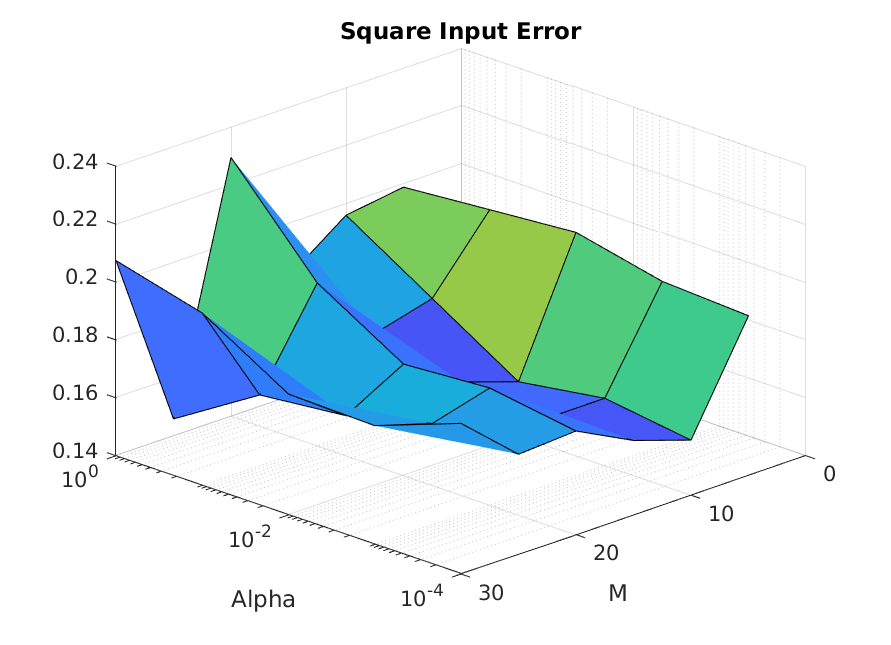
\includegraphics[width=\textwidth]{Figures_Clean/figure_square_T_0.25.png}
            \caption{Clean - 0.25 s}
            \label{fig:clean_square_025}
        \end{subfigure}
        \hfill
        \begin{subfigure}[b]{0.3\textwidth}
            \centering
            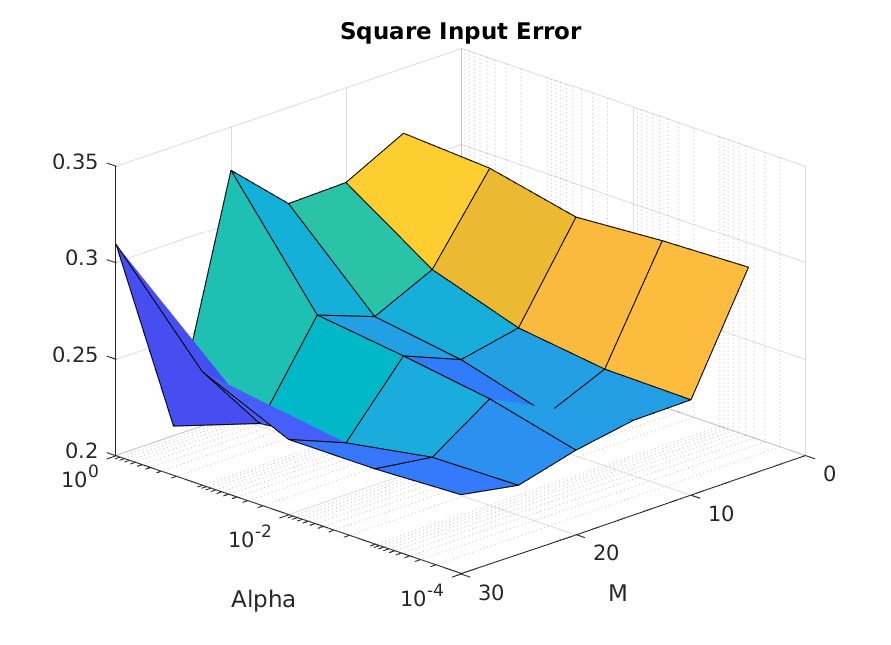
\includegraphics[width=\textwidth]{Figures_Clean/figure_square_T_0.50.png}
            \caption{Clean - 0.50 s}
            \label{fig:clean_square_050}
        \end{subfigure}
        \hfill
        \begin{subfigure}[b]{0.3\textwidth}
            \centering
            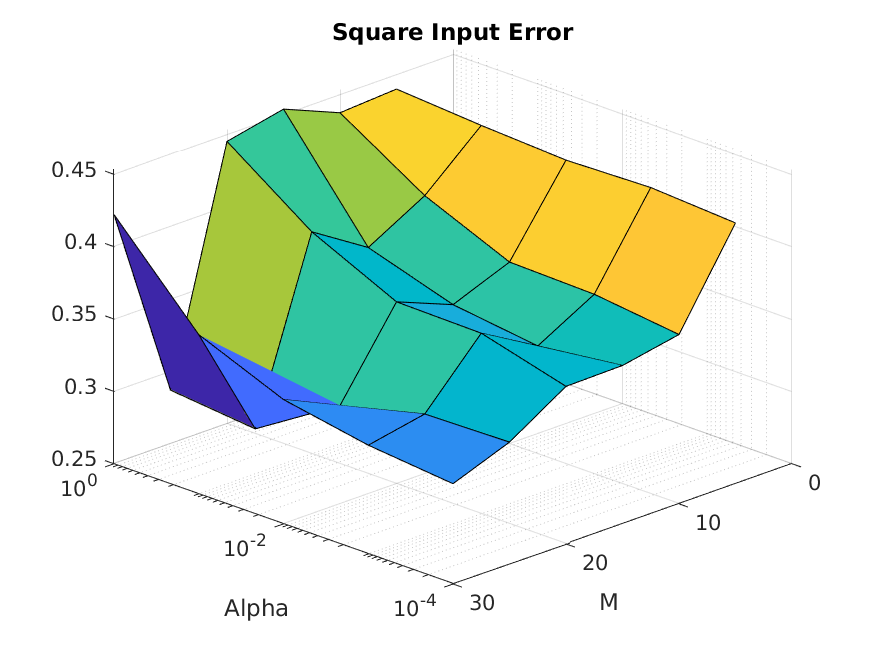
\includegraphics[width=\textwidth]{Figures_Clean/figure_square_T_1.00.png}
            \caption{Clean - 1.00 s}
            \label{fig:clean_square_100}
        \end{subfigure}
        \\
        \begin{subfigure}[b]{0.3\textwidth}
            \centering
            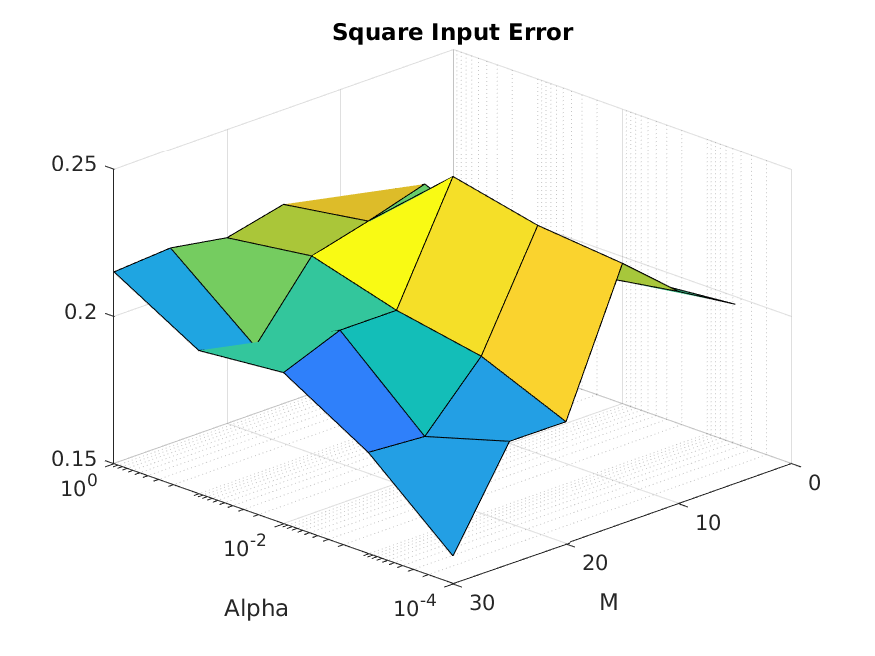
\includegraphics[width=\textwidth]{Figures_Noisy/figure_square_T_0.25.png}
            \caption{Noisy - 0.25 s}
            \label{fig:noisy_square_025}
        \end{subfigure}
        \hfill
        \begin{subfigure}[b]{0.3\textwidth}
            \centering
            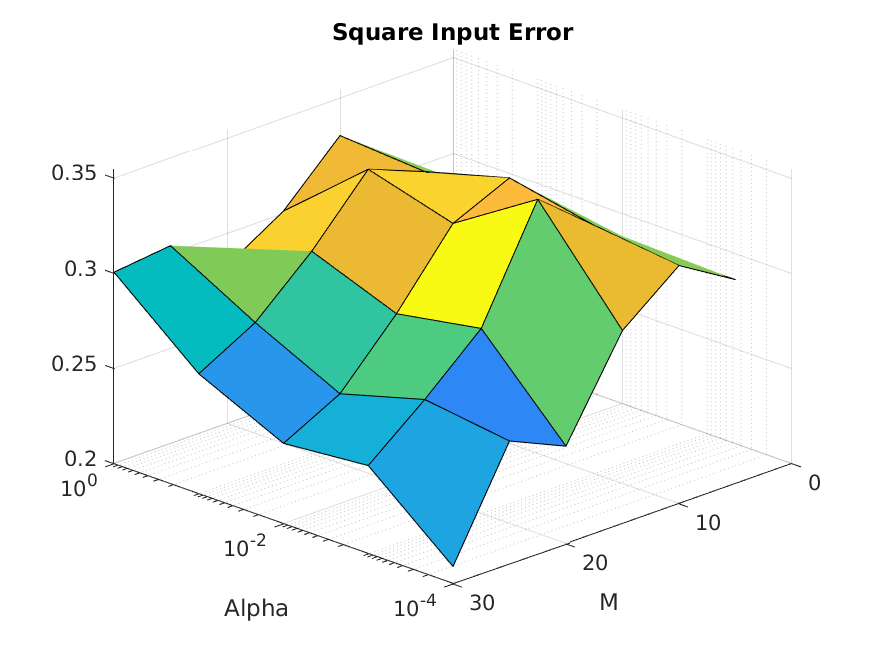
\includegraphics[width=\textwidth]{Figures_Noisy/figure_square_T_0.50.png}
            \caption{Noisy - 0.50 s}
            \label{fig:noisy_square_050}
        \end{subfigure}
        \hfill
        \begin{subfigure}[b]{0.3\textwidth}
            \centering
            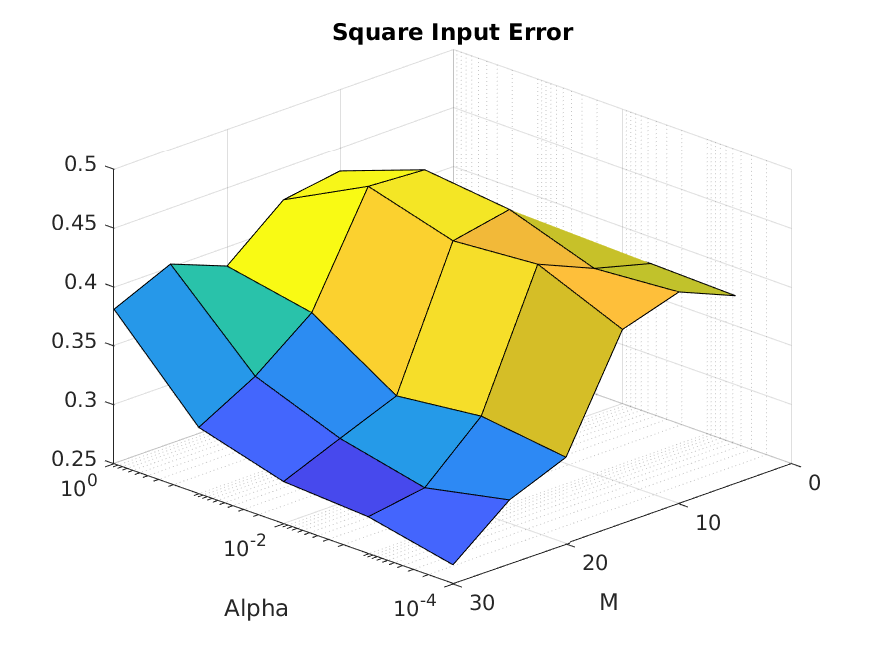
\includegraphics[width=\textwidth]{Figures_Noisy/figure_square_T_1.00.png}
            \caption{Noisy - 1.00 s}
            \label{fig:noisy_square_100}
        \end{subfigure}
        \label{fig:clean_square}
    \end{figure}
\end{frame}


\section{Conclusions}

\begin{frame}[allowframebreaks]{Conclusions}
    \begin{itemize}
        \item Prediction error can be visibly reduced by increasing the amount of observable functions; nevertheless, this trend becomes quite inconsistent over a certain dictionary size, specially when it comes to the regularized problem.
        \item Interestingly enough, the optimal regularization coefficient's order of magnitude changes depending on wether or not the training data presents measurement noise, with $\num{1e-3}$ for clean data and $\num{1e-2}$ for noisy data. Furthermore, noisy training data consistently yields better results for longer time-spans with the highest dictionary sizes evaluated and forced input. More data or different methodologies are required in order to give an explanation to this phenomenon.
        \item Despite the error trend being consistent with the operator parameters (both in regularization and dictionary size), the article results have not been achieved yet. Considering that the biggest accuracy jump so far was obtained by changing the basis function structure, further tests with different observable functions are proposed.
        \item Even though variating the observable centers does affect performance, it's better to have an even spacing over the random square than to select points from the dataset trajectories, as evidenced by the new errors and the necessity of manual intervention to get stability.
    \end{itemize}
\end{frame}

\end{document}